\documentclass[sigconf]{acmart}

\usepackage{graphicx}
\usepackage{hyperref}
\usepackage{todonotes}

\usepackage{endfloat}
\renewcommand{\efloatseparator}{\mbox{}} % no new page between figures

\usepackage{booktabs} % For formal tables

\settopmatter{printacmref=false} % Removes citation information below abstract
\renewcommand\footnotetextcopyrightpermission[1]{} % removes footnote with conference information in first column
\pagestyle{plain} % removes running headers

\newcommand{\TODO}[1]{\todo[inline]{#1}}

\begin{document}
\title{Big Data Analytics in factors affecting Bitcoin}


\author{Ashok Kuppuraj}
\orcid{1234-5678-9012}
\affiliation{%
  \institution{Indiana University}
  \streetaddress{}
  \city{Bloomington} 
  \state{Indiana} 
  \postcode{43017-6221}
}
\email{akuppura@iu.edu}


% The default list of authors is too long for headers}
\renewcommand{\shortauthors}{G. v. Laszewski}


\begin{abstract}
Pricing of Blockchain based cryptocurrencies are like a black box, as per theory the pricing compared to U.S dollar is based on a number of transactions however lot other factors like Dollar price, social media, Online threats supersede the transaction count. Big data and Analytics helps to identify the metrics impacting this variation and identify the correlation between them.
\end{abstract}

\keywords{i523, hid324, Big data, Predictive analytics, Random Forest, correlation, Blockchain, Bitcoin, Ethereum}


\maketitle

\section{Introduction}
The start of the 21st century witnessed the evolution of various disruptive technologies, right from Bigdata, IoT, VR to Blockchain. When it comes to the blockchain, the sole winner is Bitcoin, with the growth rate of over 1327 percent \cite{coingrowth:online}, Bitcoin is disrupting the way banking system works. As the Bitcoin grows the acceptance and adoption grow along with that. Similar to any other currency in the world, the Bitcoin's price deviates widely towards the positive side which created the opportunity for investment in it. Even though the same is not widely accepted everywhere, there is a grace to own Bitcoin citing its growth rate. Though the transaction counts haven't grown up, the retention of the coin has grown up making it a Digital Gold \cite{Retain:online}.


\section{Bitcoin}
Bitcoin is a progressed cryptographic cash and portion structure that is completely decentralized, which implies it relies upon peer-to-peer trades with no bureaucratic oversight. Trades and liquidity inside the framework are somewhat based on cryptography. The concept was first introduced in 2009 \cite{Bitcoin} and is at this moment a prospering open-source gathering and portion sort out. In perspective of the uniqueness of Bitcoin's portion tradition and its creating choice, the Bitcoin condition is grabbing stacks of thought from associations, clients, and monetary experts alike. Specifically, for nature to thrive, we need to recreate budgetary organizations and things that starting at now exist in our traditional, fiat cash world additionally, make them available and uncommonly specially fitted to Bitcoin, and other rising computerized types of cash.
In technical terms, Bitcoin's is a shared ledger or a database running by a set of clusters, as the clustering is involved, a competition is set for the individual machines to acquire and update the ledger. The competition is in terms of hashing problem. The hashing needs multiple GPU's to perform validations and update the ledger. This competition eliminates the slower machines to be part of the network and improve the infrastructure's capacity, only by winning the competition a machine can be awarded some Bitcoin as an incentive. Since one machine cannot process the competition problem, a set of peers come together to form a Mining pool and share their capacity and the incentives. We can gather useful mining statistics information from these mining pools.
 
 \section{Price prediction}
 The Bitcoin market's cash-related basic is, clearly, a securities trade. To support money related to reward, the field of stock exhibit gauge has turned out to be over the earlier decades and has all the more starting late exploded with the presence of high-repeat,low-dormancy trading hardware joined with solid machine learning figurings. Henceforth, it looks good that this desire is imitated in the domain of Bitcoin, as the framework expands more conspicuous liquidity and more people develop an excitement for placing profitably in the structure. To do accordingly, it is essential to utilize machine learning advancement to foresee the cost of Bitcoin\cite{stock}.
 
 
 \subsection{Data Source}
 As Bitcoin is a decentralized and a transparent system, all the source of data can be gathered from the peer-to-peer networks. This peer-to-peer network is called as Bitcoin-mining pool \cite{1:online}.The rate of block creation is adjusted every 2016 blocks to aim for a constant two week adjustment period (equivalent to 6 per hour.) The number of Bitcoins generated per block is set to decrease geometrically, with a 50 reduction every 210,000 blocks, or approximately four years. The result is that the number of bitcoins in existence is not expected to exceed 21 million \cite{2:online}.
The true source of data for Bitcoin analysis would be from Bitcoin mining pool. Coinbase is one of the main member bitcoin pool from which we can gather mining statistics. Here the data is sourced from a data service called Quandl. Quandl provides the variety of data services in the form of https web services. As we are in the process of identifying the features impacting Bitcoin's price fluctuations, not only the transaction volume impacts, even the popularity and people's trend towards it impact the price of the coins. Hence, data from Google is also gathered. As a currency's price also been altered by its exchange, supply, and demand, Ethereum's price data and transactional data is also acquired from Ethereum's exchange point.
With all these data sources, we analyze the features impacting the Bitcoin's market price. 
 
 
 \subsection{Feature selection}
 Feature selection is one of the vital steps in any meaningful analysis of an expected outcome. A set of features have been selected to analyze its interdependence with Bitcoin's evaluation. The features selected based on three wide areas, the first is Bitcoin mining data, second is social data and the last one is exchange data.
 The internal activities in the Bitcoin's infrastructure definitely reflect the changes or the fluctuations in the Bitcoin's network, Bitcoin's mining data is gathered from Coinbase. This is extracted from the Web service API provided by Quandl.com\cite{3:online}. By making a REST call, CSV files containing the Historical data is downloaded and processed.
 The second is the social data, which is extracted as a static data from Google trends \cite{google:online}, the main reason behind this data is when the popularity grows people tend to know or show interest in being part of the growth. With the impressive growth of more than 1000 percent in a year, this is considered as an important data.
 The last one is the exchange data, as a currencies price is directly proportional to the supply and demand, the supply of the currency can be impacted by the exchange to other currencies or commodity \cite{4:online}. Ethereum is known to show a similar pattern in terms of growth and deviations\cite{Ethereum:online}. Hence, there's price in US dollars and transaction volume is considered one of the features.

\section{Big data in Feature Analysis and Algorithm's execution}
Feature extraction, transformation, and prediction can be synonymous with a conventional ETL methodology. Though few of the extraction is handled manually and the volume is comparably low, it is assumed that the data volume will be increased by modifying the extraction to real-time systems. When the extraction systems are changed, our code must be able to handle streaming data which can be related to "variety and volume " of the data. The next step is validating the data for anomalies, data miss and cleanse the data of issues which is synonymous with data cleansing. The later one is data processing, which includes data processing with multiple iterations and permutation consuming a lot of memory and other resources. These processing needs lead us in adopting Big data technologies in the entire lifecycle of the implementation.

\subsection{Execution with Apache Spark}
''Apache Spark is a fast and general-purpose cluster computing system. It provides high-level APIs in Java, Scala, Python and R, and an optimized engine that supports general execution graphs''. It also provides extensive support to Machine learning libraries(MLlib) and to streaming through Spark Streaming. The in-memory processing is implemented with the help of Resilient distributed dataset (RDD) \cite{5:online}.

\begin{figure}[!ht]
  \centering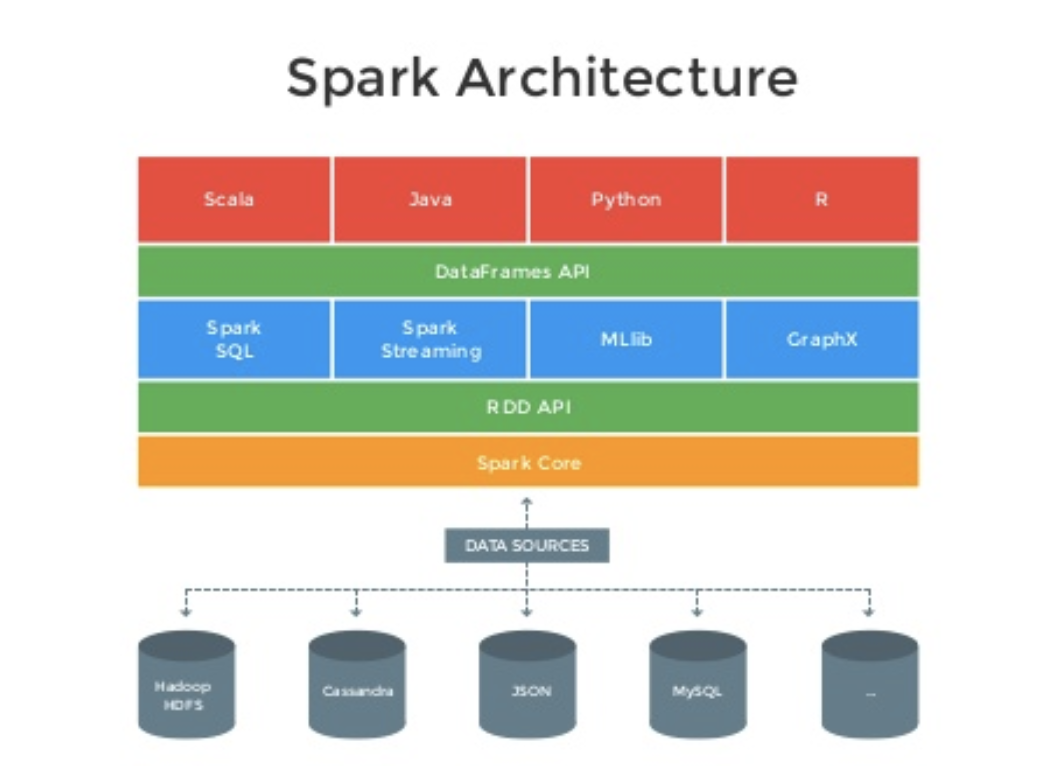
\includegraphics[width=\columnwidth]{images/Sparkarchic.png}
  \caption{Spark Architecture}
\end{figure}

Spark's basic abstraction is Resilient Distributed Dataset (RDD), which is a fault tolerant partitioned data encapsulation datatype. RDDs are lazily evaluated, hence a Directed Acyclic Graph is implemented to persist the state of the RDDs at each stage. With RDD, Spark can execute the transformation in parallel with fault tolerance. This implementation widely differentiates from conventional Python implementation which lacks this advanced logic.  

Here, we have used Apache's Spark 2.2 to implement all the ETL functionality. Spark is installed is the local system along with Anacondas, so Spark libraries can be consumed inside Python shell. To consume and process Pyspark libraries, sparkcontext is created which initiates the driver program. The spark context is bootstrapped with SQL and Spark session libraries so that Spark RDD and Data frames could be accessed under a single window.

As the abstract describes the necessity of the features impacting bitcoin's price, the best metric to identify the relation between bitcoin's values and its features is by identifying the correlation matrix provided by Spearman. Spearman's function describes the relationship between two variable using a monotonic function\cite{Spearman9:online}. Apart from identifying the correlation, these features can be modeled to predict the value of the dependent variable - Bitcoin's value. The algorithm chose are Random forest and gradient boosted regression.

\section{Implementation}
The actual implementation starts with gathering source data with features already discussed the prior topic, upon data extraction, it is cleansed with missing data and standardized to mix and match data from multiple sources. All the data manipulation is done either in Pyspark dataframe or pyspark RDDs. The visualization is provided by Matplotlib.

\begin{figure}[!ht]
  \centering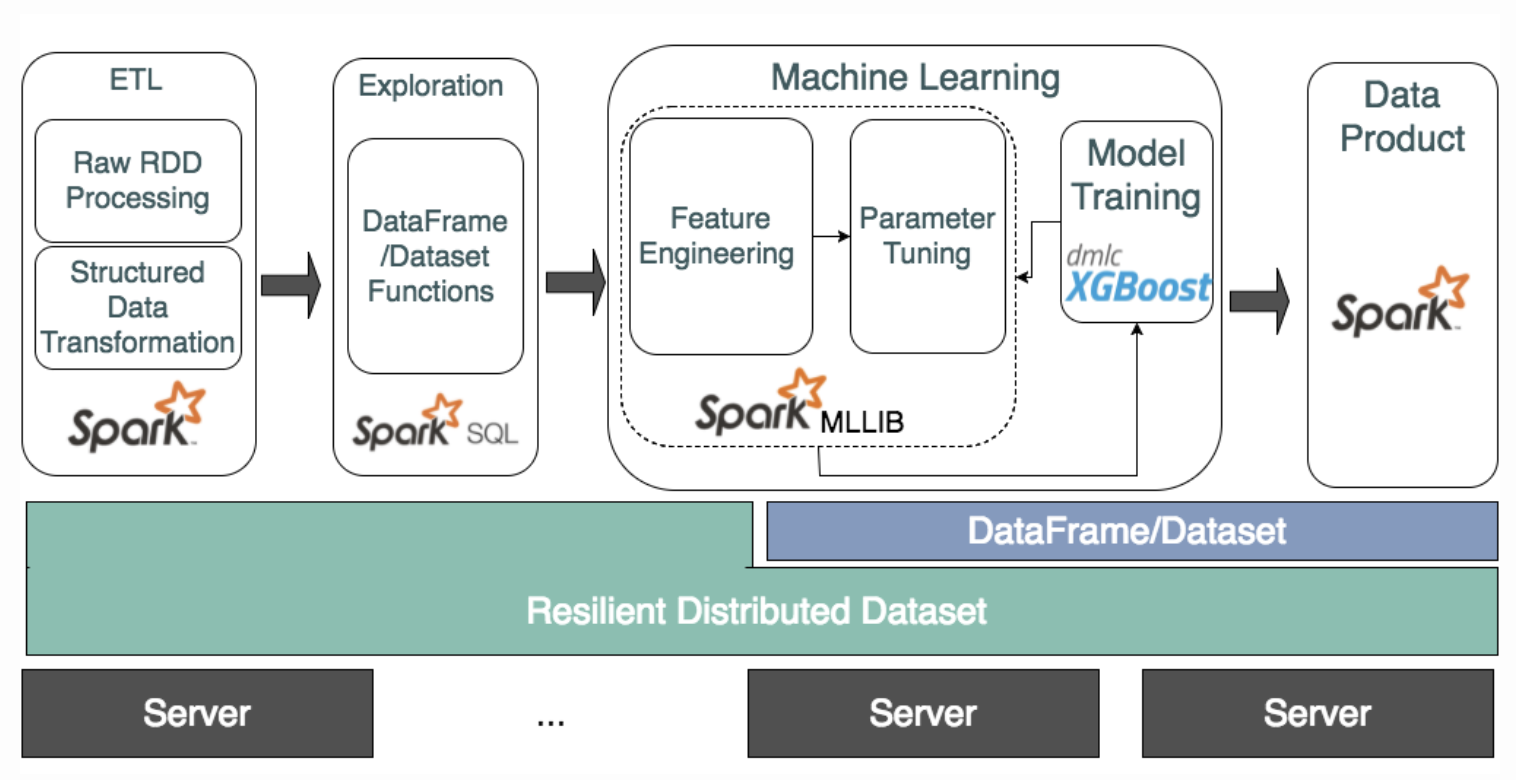
\includegraphics[width=\columnwidth]{images/Projectflow.png}
  \caption{Project Architecture on Spark}
  \label{Architecture:spark}
\end{figure}

As shown in figure \ref{Architecture:spark}, the extracted data is loaded to Pyspark RDD and then converted to Pyspark dataframe.Pyspark dataframe is selected to increase the performance of the data processing even though Pyspark dataframe API is not equipped with rich functionalities similar to Pandas dataframe and Pyspark dataframe can execute the transformations in parallel whereas Pandas cannot. 

\subsection{Technologies}
Technologies and tools used in this projects are
\begin{itemize}
\item Python 2.7 
\item Pyspark 2.2
\item Jupyter 5.0.0
\end{itemize}


\subsection{Data Extraction}
The data is sourced from Quandl.com, a public data service for various types of data, Bitcoin's mining data from 2015 till current date from Coinbase's mining pool. The data is in CSV format with Bitcoin's transaction details and its corresponding date associated with it.

The second set of data is from Etherscan, an open source portal for Ethereum transaction details, from which the transaction count and the price in US dollars are extracted.

The third dataset is about the people's trends on Bitcoin's popularity from Google, the granularity of this data is on weekly basis, hence it has to transformed statistically to fit into our model.

The first data set is programmatically downloaded with an API call with a private key authenticating it. {\em wget } is used in downloading the data within Shell script.
The later ones are downloaded manually from Google and Etherscan sites manually. The volume of the dataset is low, however, the volume increases as the consumption are initiated in real-time.

\begin{figure}[!ht]
  \centering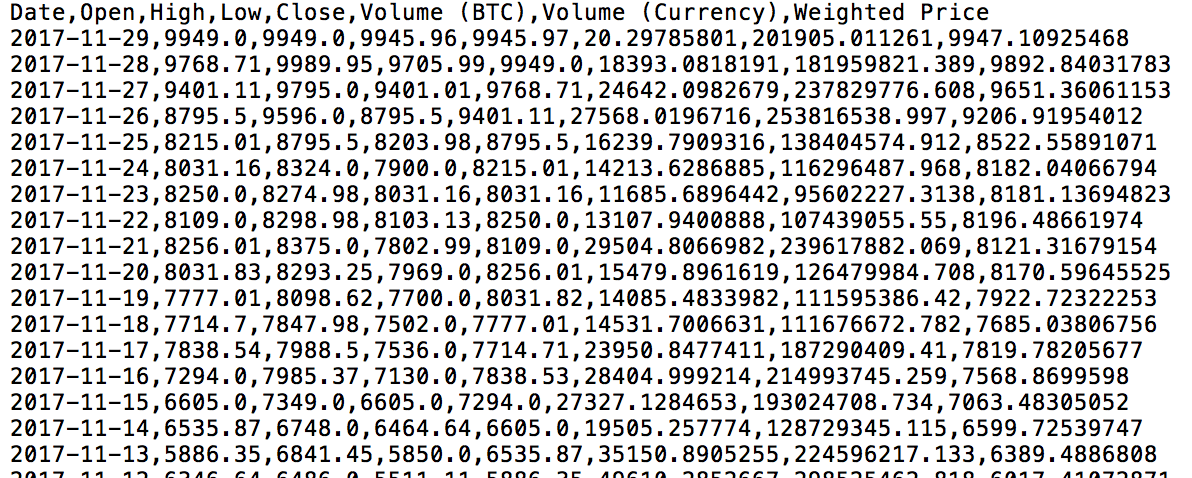
\includegraphics[width=\columnwidth]{images/Source1data.png}
  \caption{Bitcoin mining statistics data}
  \label{}
\end{figure}

\subsection{Data Cleansing}
The data cleansed with multiple Python and feature cleansing libraries in Python and Pyspark. Major efforts of cleansing are needed to standardize the date columns from all the data sources. The date format was in the different format in different sources. To stitch back all the data points, DateTime libraries were used and joined with a single standard format. Another important activity in the cleansing is data miss. For some instance data points, the values are missing resulting in incorrect predictions and correlations. To resolve these missing values, Imputer\cite{imputer:online} functionality is used from feature library of Apache Spark. The imputer is an Imputation estimator for completing missing values, either using the mean or the median of the columns in which the missing values are located. The input to this function is dataframe columns and output are renamed dataframe columns. The processing happens in-memory with the spark.

\subsection{Data Visualization}
The visualization is provided in the form of plots. In Python, we have to use Matplot Libraries to plot all the prediction and correlation graphs.


\section{Spearman's correlation}
Spearman's correlation function is used to identify the correlation between Bitcoin's price and the features selected. In Spark, a separate function is defined to calculate Spearman's correlation. The input is in Pyspark RDD's and the output value is returned between -1 to +1. The positive ratio indicates the feature is directionally proportional and the negative values indicate indirect proportionality.

The below table describes the correlation of Bitcoin's price with the features. Surprisingly the transaction count of the Bitcoin is very less related to its value against US dollars. Whereas the

Spearman's Correlation on selected features are :
\begin{itemize}
\item btc-vol     :0.348540857386 
\item high        :0.998581861669 
\item low         :0.995190604708 
\item open        :0.997943642437  
\item Google-trend:0.260343238604  
\item ETH price   :0.68683414787  
\item ETHTRAN     :0.720031468617
\item btc-price-Label:1.0 
\end{itemize}

\begin{figure}[!ht]
  \centering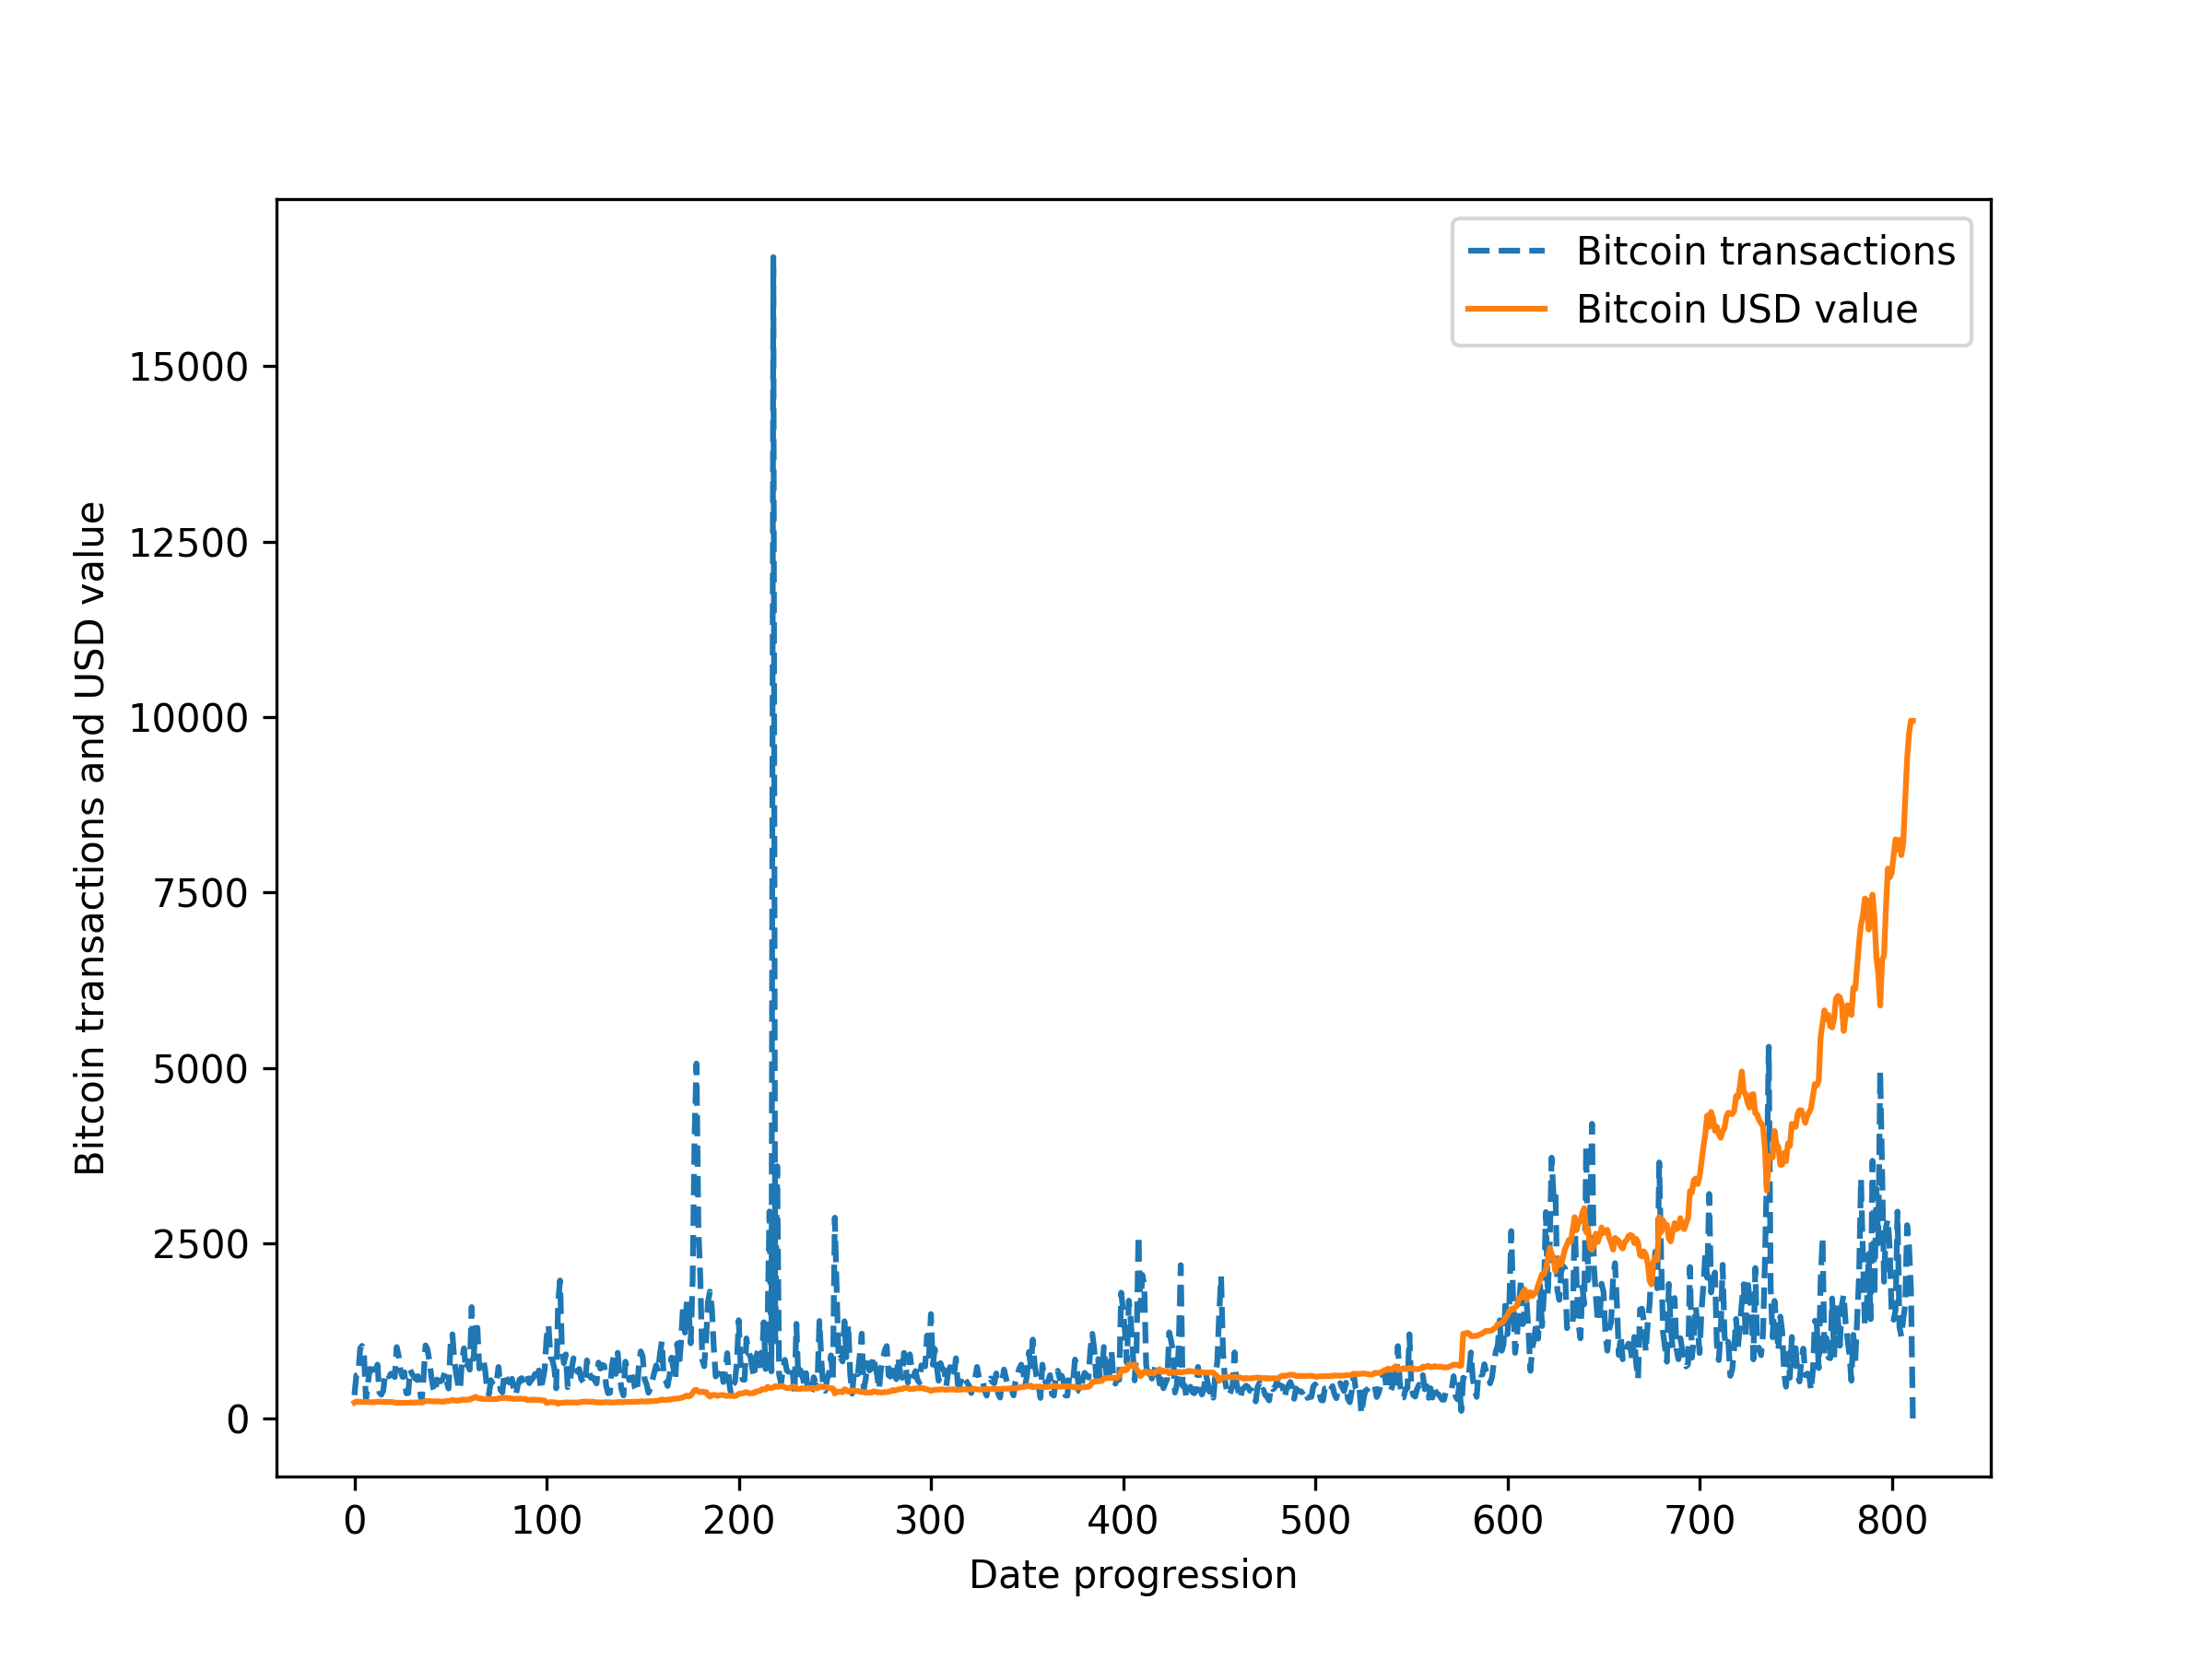
\includegraphics[width=\columnwidth]{images/BTC-prcvsBTC-trans.png}
  \caption{BTC Transaction and USD value - 0.348540857386 }
  \label{1}
\end{figure}

The Figure\ref{1} describes the correlation between Bitcoin transaction count and its value. Or in other perspectives, the transaction count is consistent and due to the increase in price people started buying Bitcoins leading to volatility.

\begin{figure}[!ht]
  \centering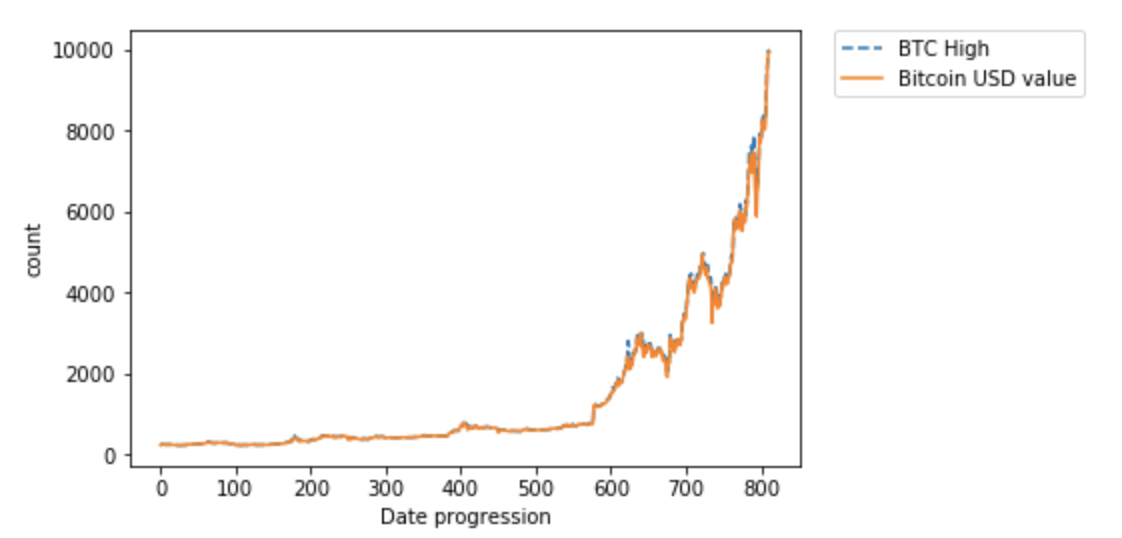
\includegraphics[width=\columnwidth]{images/High.png}
  \caption{Bitcoin Highest exchange value and Closing value - 0.998581861669  }
  \label{2}
\end{figure}

The Figures \ref{2},\ref{3} and \ref{4} describes the correlation between open, low and high prices of Bitcoin on the recorded date. This is obvious that the closing price is highly correlated with them.

\begin{figure}[!ht]
  \centering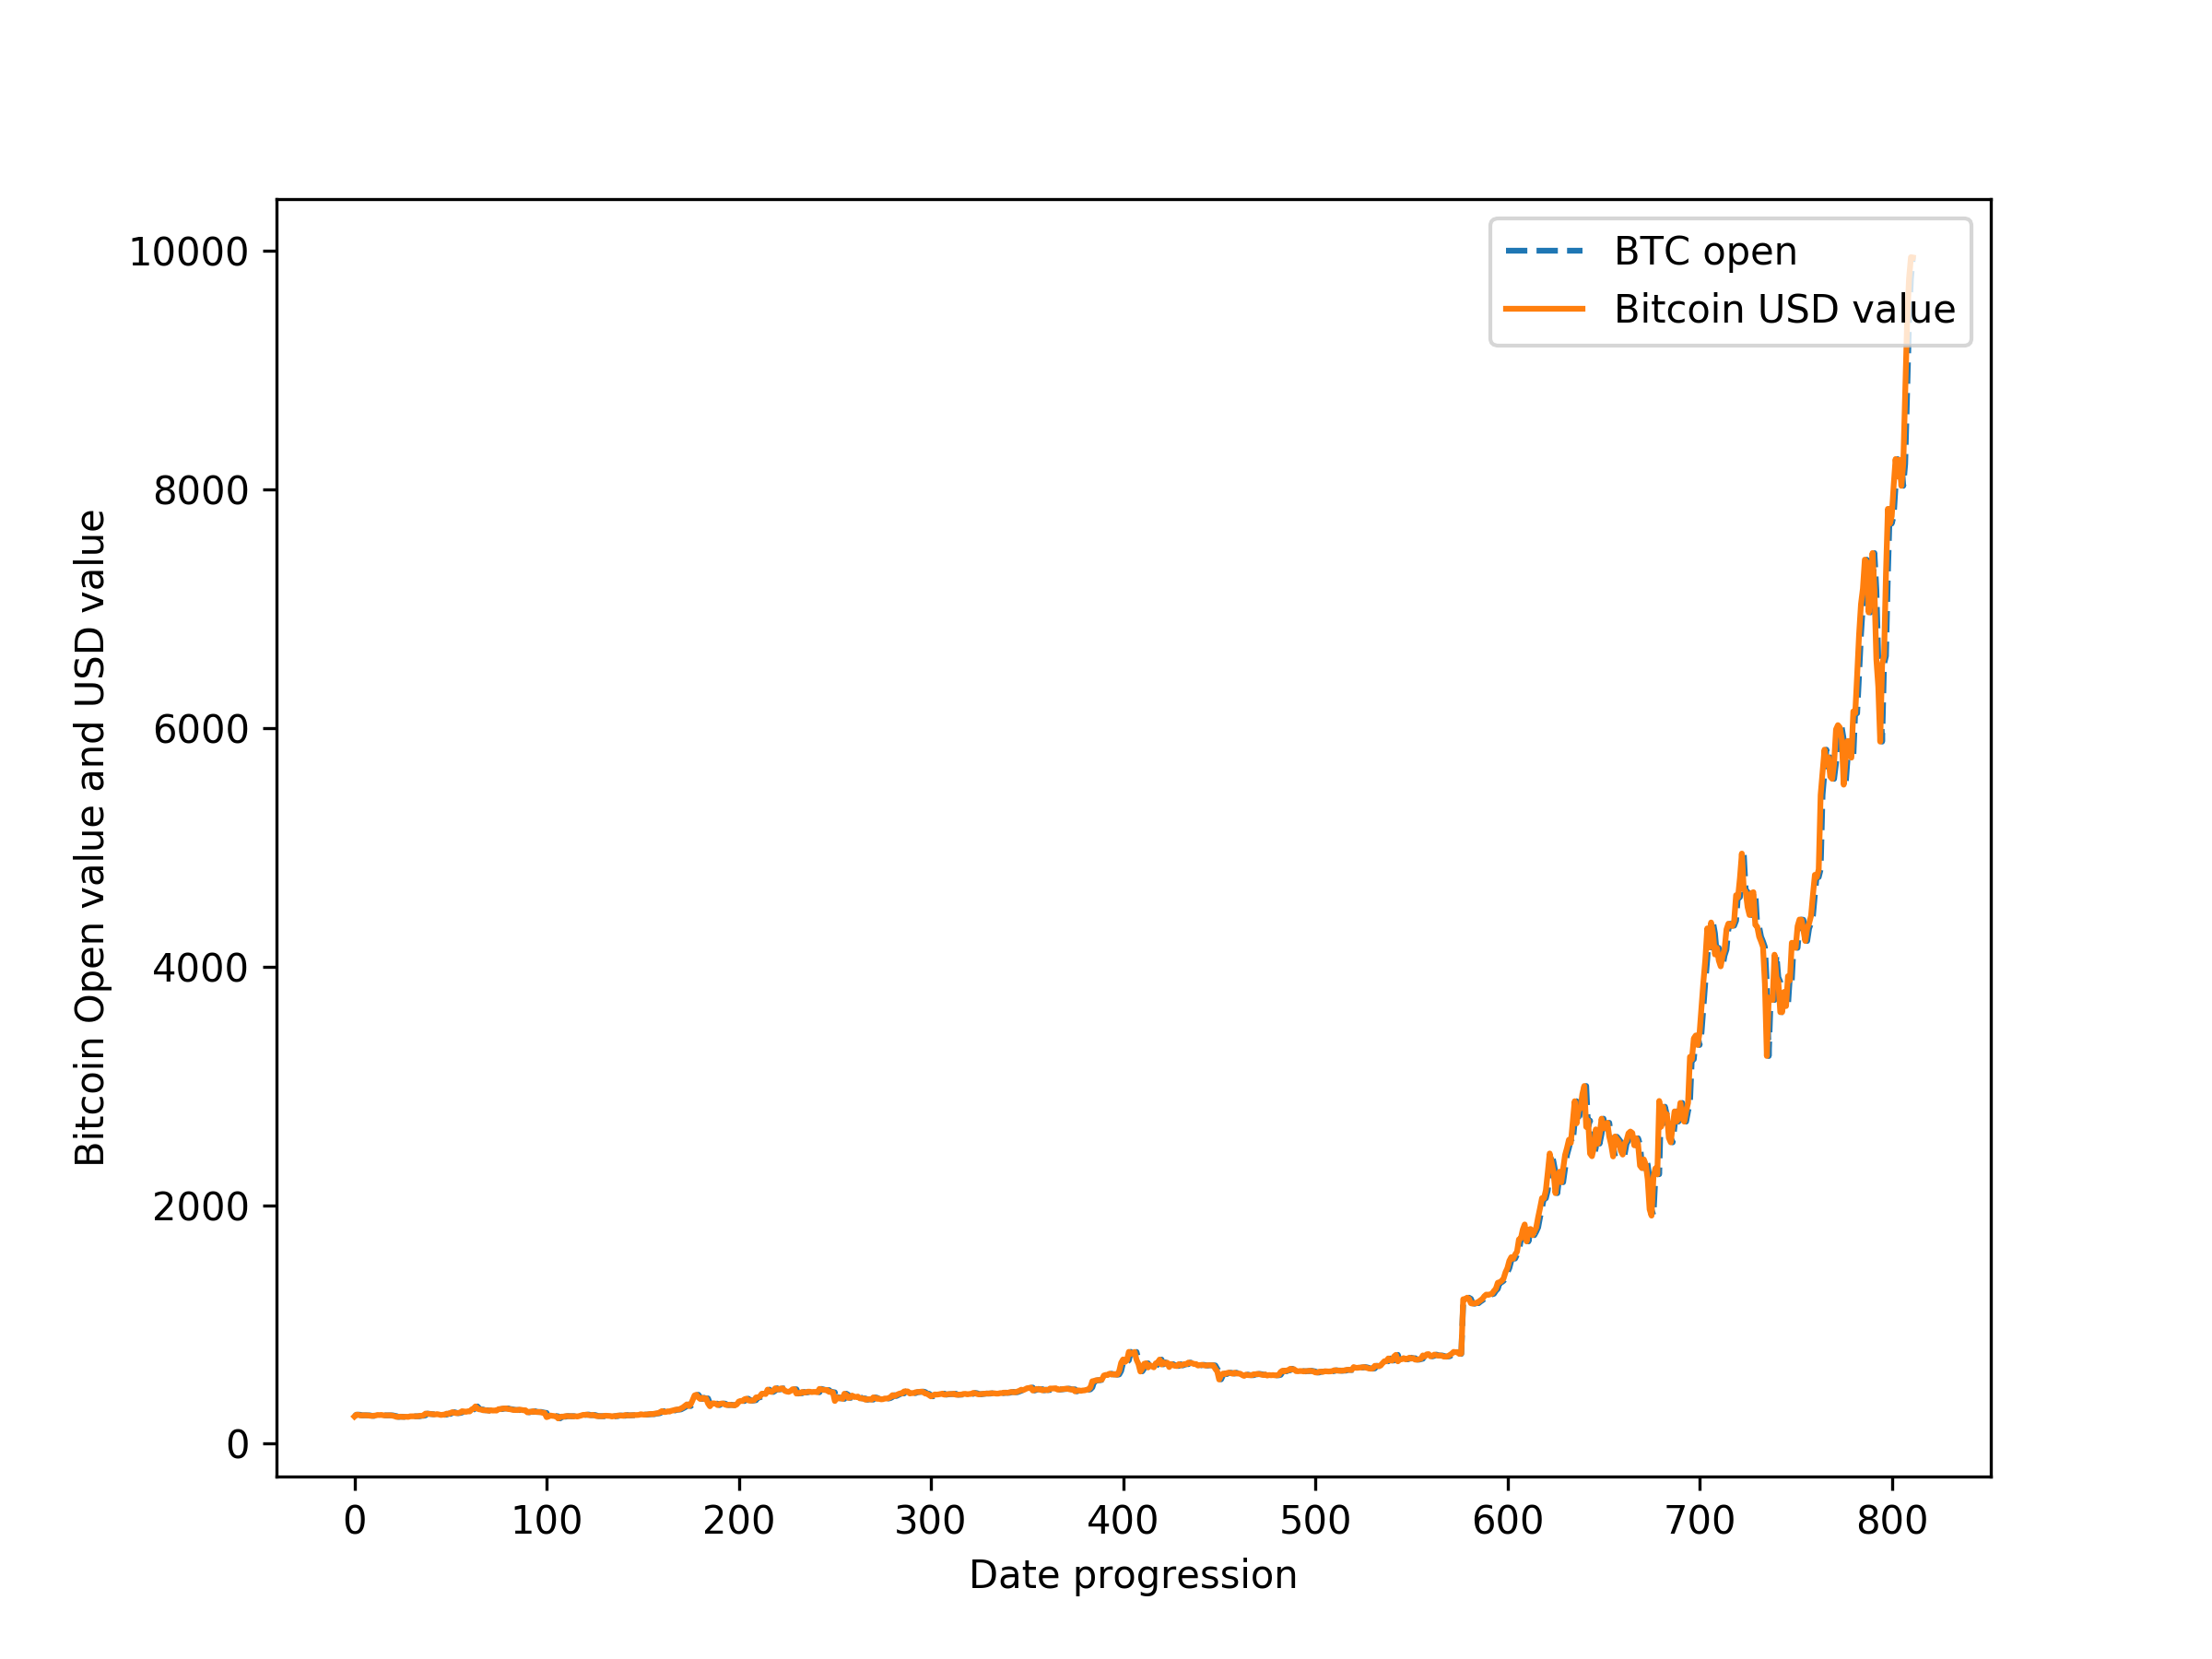
\includegraphics[width=\columnwidth]{images/Open.png}
  \caption{Bitcoin Lowest exchange value and Closing value - 0.995190604708  }
  \label{3}
\end{figure}

\begin{figure}[!ht]
  \centering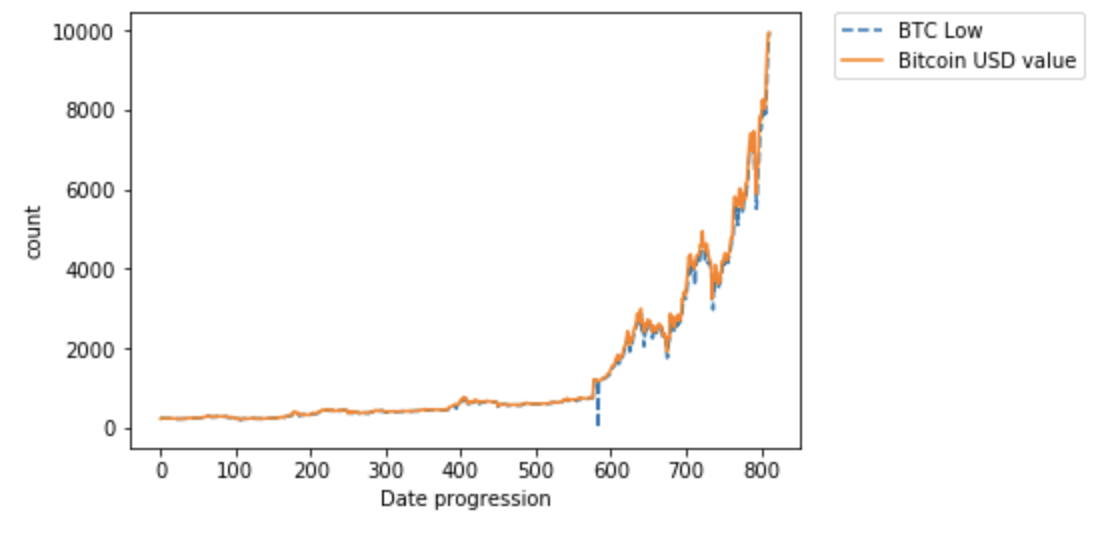
\includegraphics[width=\columnwidth]{images/low.png}
  \caption{Bitcoin Opening exchange value and Closing value - 0.997943642437}
  \label{4}
\end{figure}


\begin{figure}[!ht]
  \centering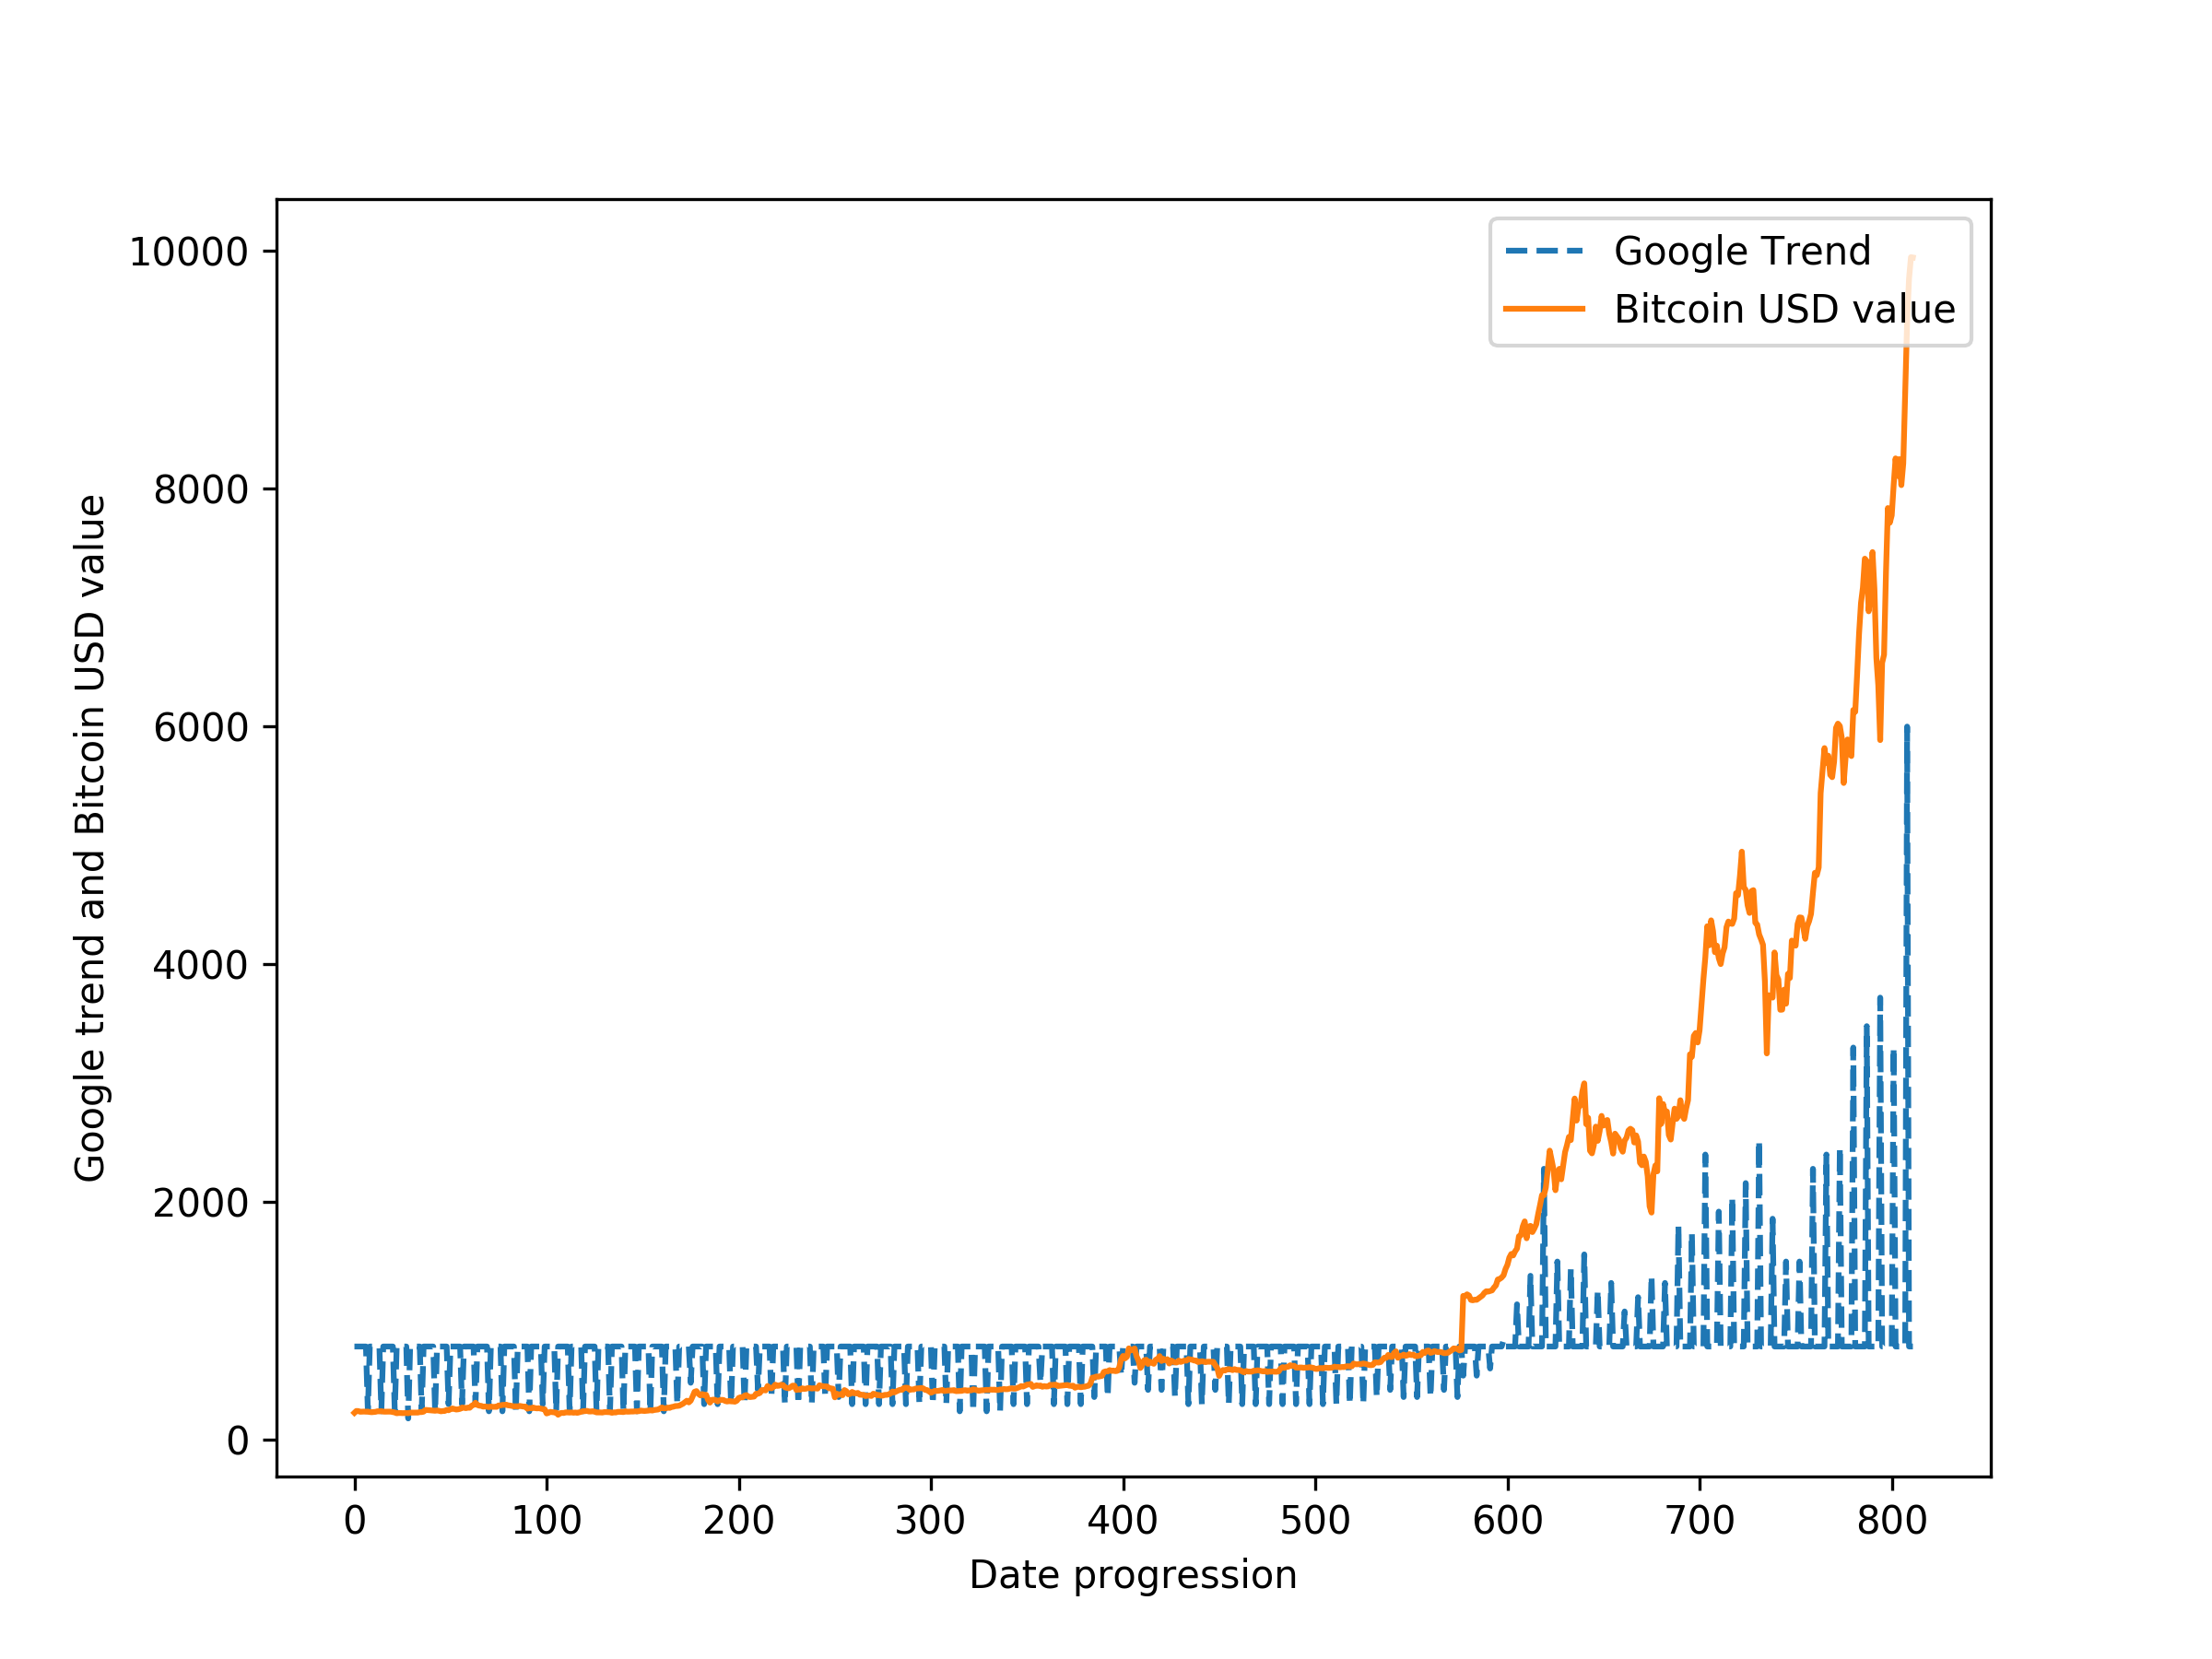
\includegraphics[width=\columnwidth]{images/googletrend.png}
  \caption{Bitcoin USD value and Google search trend - 0.260343238604}
  \label{5}
\end{figure}

As described in figure \ref{5}, the correlation plot provides the pattern between the search trends and the hike in price, which is clearly evident.

\begin{figure}[!ht]
  \centering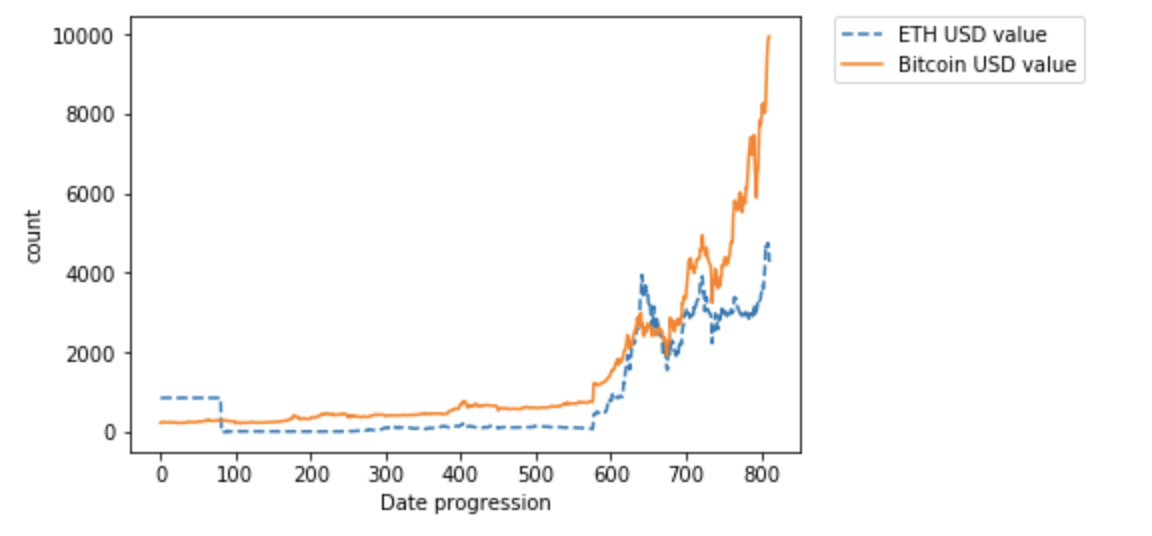
\includegraphics[width=\columnwidth]{images/ethvalue.png}
  \caption{ETH price and BTC price - 0.68683414787 }
  \label{6}
\end{figure}

\begin{figure}[!ht]
  \centering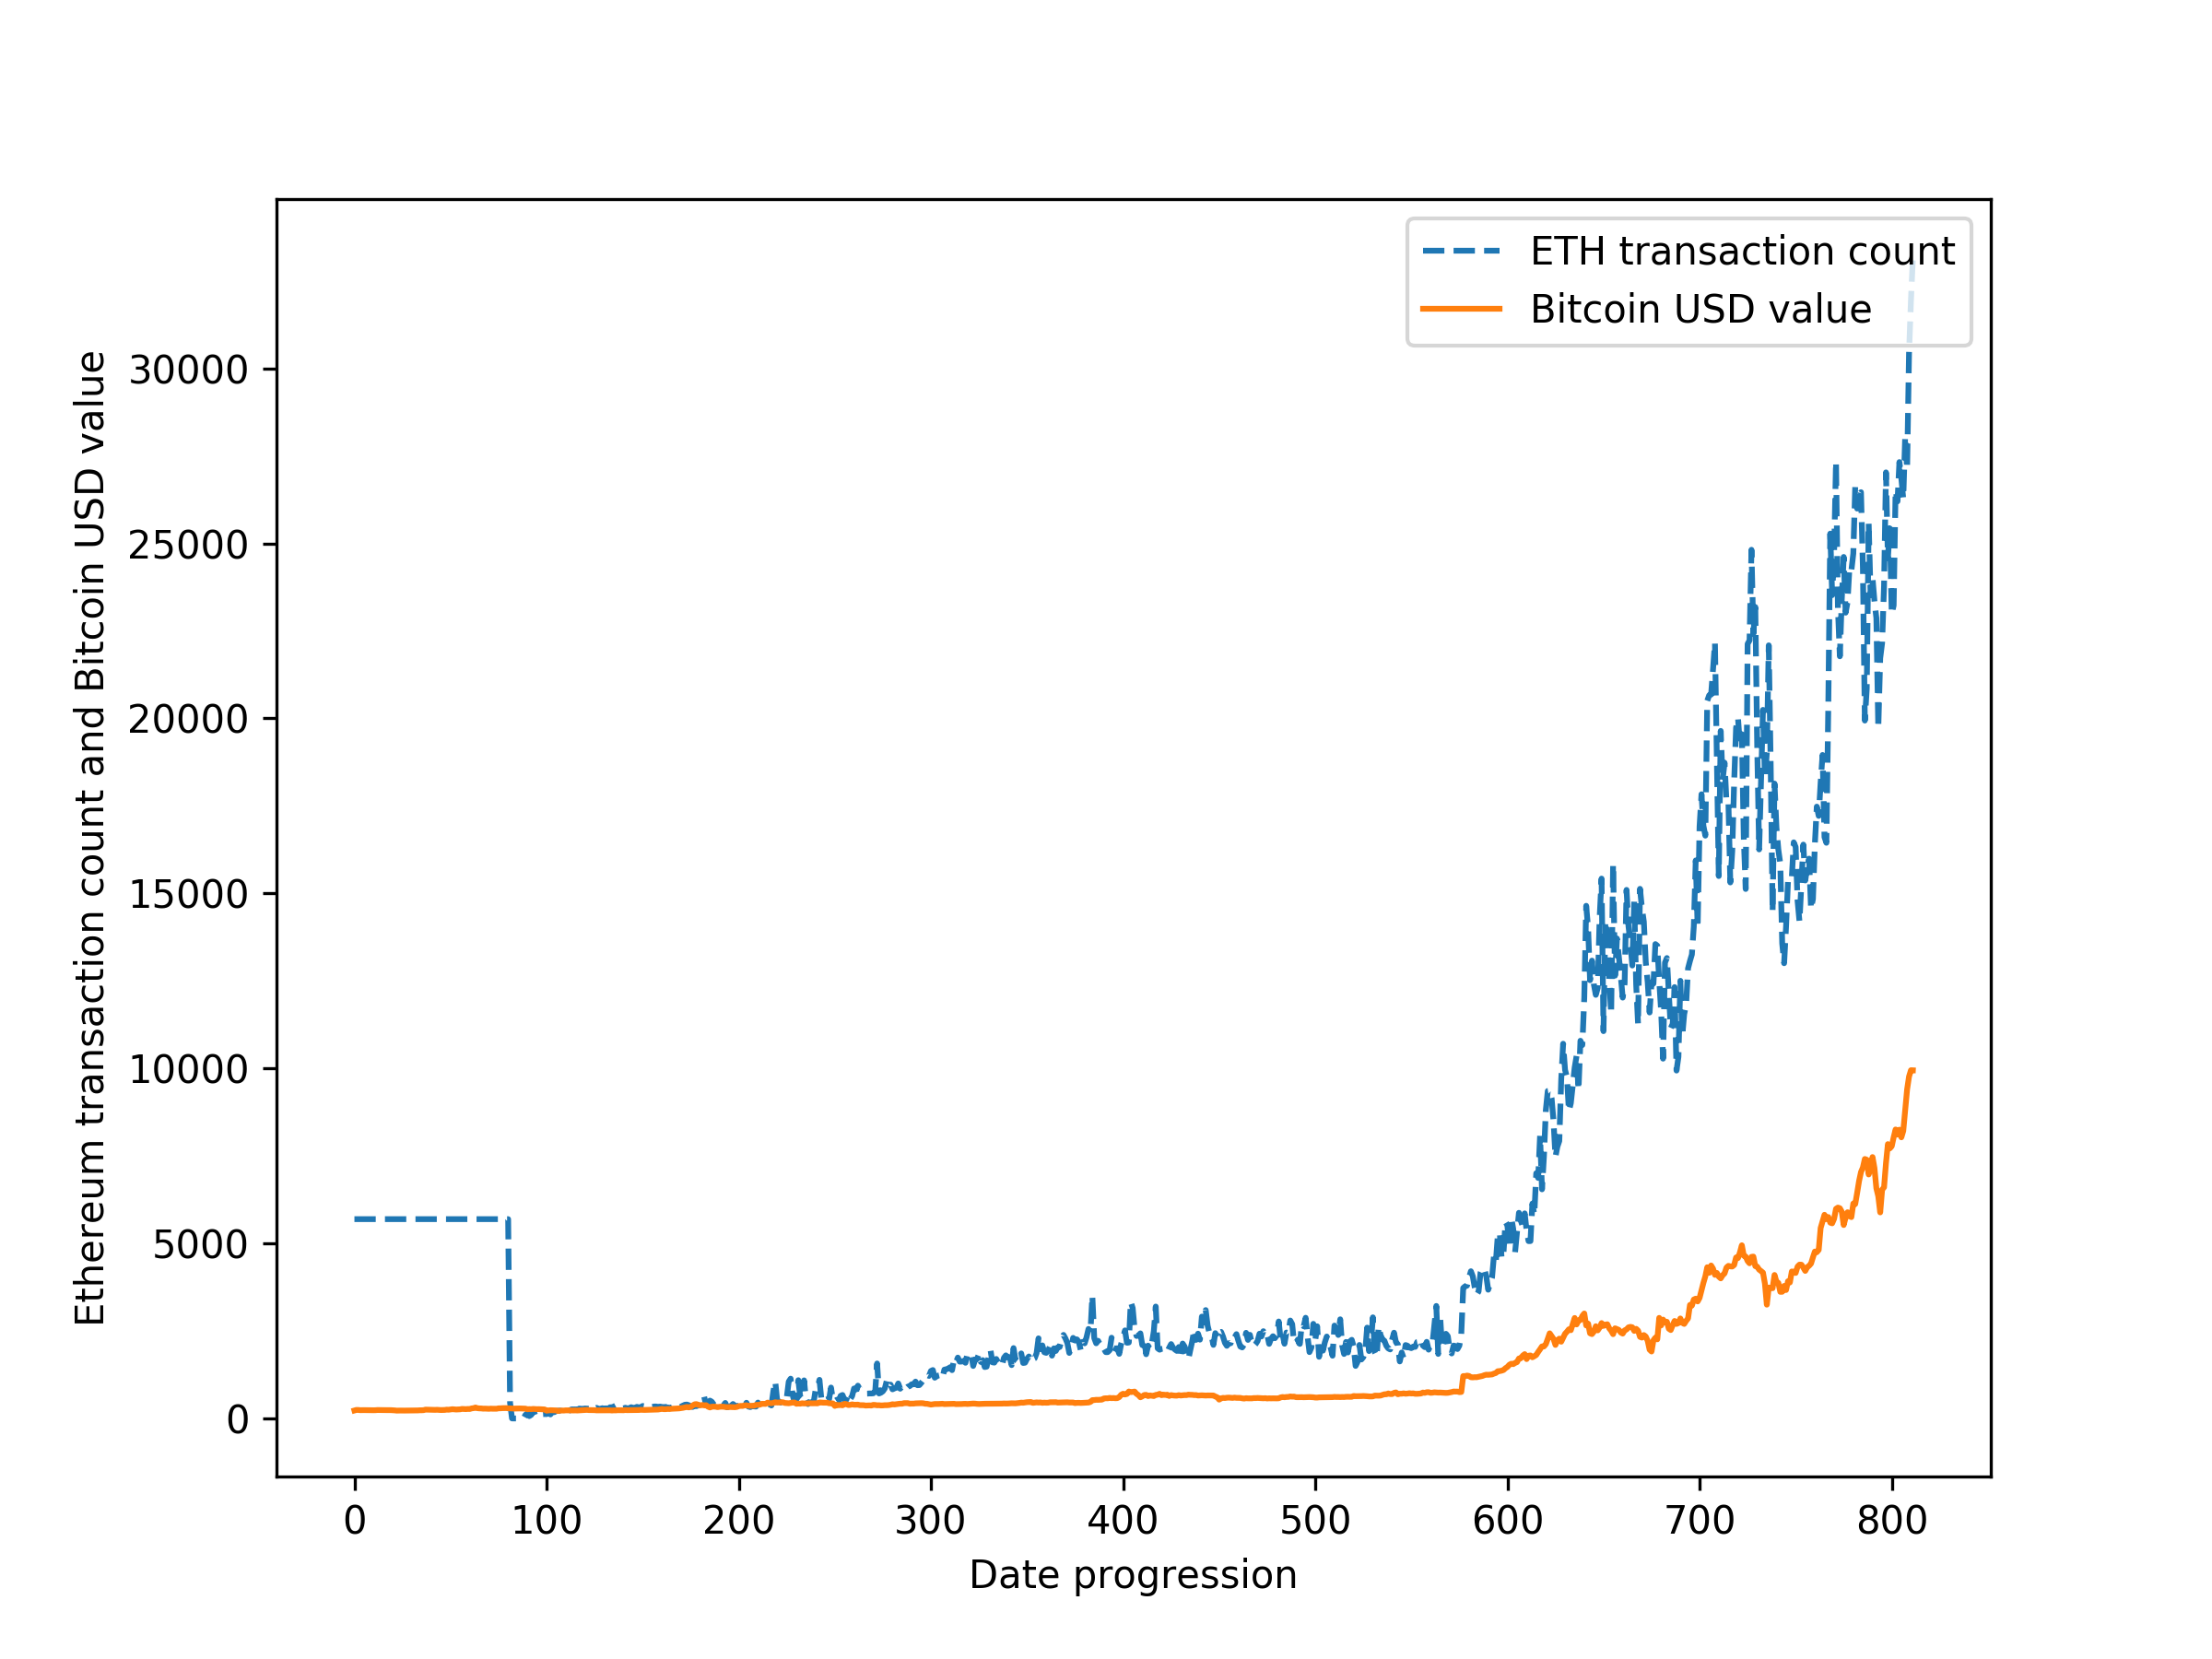
\includegraphics[width=\columnwidth]{images/ethtrancount.png}
  \caption{ETH Transaction volume and BTC transaction volume - 0.720031468617 }
  \label{7}
\end{figure}

Figure \ref{6} and \ref{7} describes the correlation of Ethereum's price and its transaction volumes with Bitcoin's price in which the transaction pattern of Ethereum is more similar to Bitcoin's pattern is evident. 

As far as processing is concerned, all the RDDs are cached before feeding into Spearman's correlation function, the reason being, when the RDDs are transformed multiple times, it has to calculate data lineage everytime it is computed and lineage is the basic quality of resilience in Apache Spark. If the RDDs are cached and persisted in-memory, the iteration and other transformations happen in memory avoiding costly I/O operations, this feature cannot be easily implemented when executed in conventional python libraries.


\section{Decision tree regression}
With the availability of features, we can take the processing to the next level of predicting Bitcoin's price. Here, supervised learning model is used to predict the price of Bitcoin.

\begin{figure}[!ht]
  \centering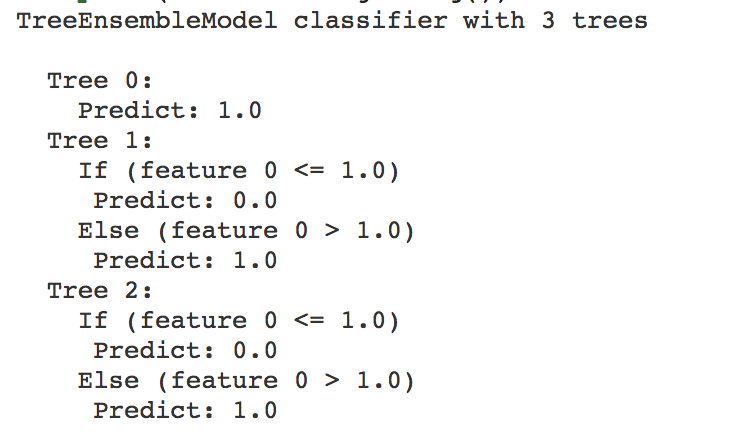
\includegraphics[width=\columnwidth]{images/Decisiontree.png}
  \caption{Sample Decision tree}
  \label{fig:8decisiongree}
\end{figure}
 

Figure \ref{fig:8decisiongree} give some basic idea of how decisions are made with the supervised decision tree based model.

Ensemble method models are derived from another base model. The base model used here is Decision trees and ensemble models are Random forest and Gradient Boosted tree(GBT) Algorithms.

Though the base model for both the algorithms is same, both are different in terms of training the dataset. GBT can train only one tree at a time whereas Random forest can train multiple trees resulting in reduced overfitting caused by GBTs.

''Random forests or random decision forests operate by constructing a multitude of decision trees at training time and outputting the class that is the mode of mean prediction (regression) of the individual trees and GBTs iteratively train decision trees in order to minimize a loss function. Like decision trees, GBTs handle categorical features, extend to the multiclass classification setting, do not require feature scaling, and are able to capture non-linearities and feature interactions''\cite{Ensemble4:online}.

All the execution is implemented in Apache Spark, hence all the transformation and processing happens in-memory, even if the data volume is high, the processing will spawn across the clusters and will be processed with consistent redundancy.

The model is implemented by first splitting the data into two sets of different volume, i.e test data and training data. The training data will be used by the model to derive the logic and the built logic will be tested with the test data for accuracy. Here, 70:30 ratio is selected for training and test data respectively. And by altering this ratio we can adjust the performance of the model.

\subsection{Random Forest}
As we are predicting Bitcoin's USD value per day, Bitcoin's price in considered as a label and all other columns are marked as features, and only the features having a decent level of correlation is marked as Features. These features are loaded into the model as Labelled Points as a Spark dataframe.

Random forest requires parameters to tune the model for the highest accuracy. Below are parameters selected for our model.
\begin{itemize}
\item Training dataset: RDD of LabeledPoint. Labels are real numbers.
\item numTrees ={\em 10}   Number of trees in the random forest.
\item featureSubsetStrategy ={\em auto}   Number of features to consider for splits at each node.
\item impurity ={\em variance }  Criterion used for information gain calculation 
\item maxDepth ={\em 30 }  Maximum depth of tree
\item maxBins {\em default }   Maximum number of bins used for splitting features
\item seed {\em default }   Random seed for bootstrapping and choosing feature subsets
\end{itemize}

With all parameters set and by tuning the model, Avg.closeness index of the algorithm is closer to 0.95. After deriving the model, the closeness/correctness of the predicted results was also analyzed and it is described in the plot given below.

\subsection{Gradient Boosted tree}
In the Gradient Boosted algorithm, the similar training and test data are used similarly to the Random Forest algorithm. Upon execution of three iterations, it is clearly evident with the closeness index that the data is little bit over-fitted with the closeness index of 0.96, slightly greater than Random forest.
The parameters used in these functions are 
\begin{itemize}
\item data  Training dataset: RDD of LabeledPoint. Labels are real numbers.
\item categoricalFeaturesInfo  Map storing arity of categorical features
\item loss  Loss function used for minimization during gradient boosting
\item numIterations  Number of iterations of boosting
\item learningRate  Learning rate for shrinking the contribution of each estimator
\item maxDepth  Maximum depth of tree 
\item maxBins  Maximum number of bins used for splitting features.
\end{itemize}

By altering the parameters, the performance of the model can be optimized.

\section{Results}

\begin{figure}[!ht]
  \centering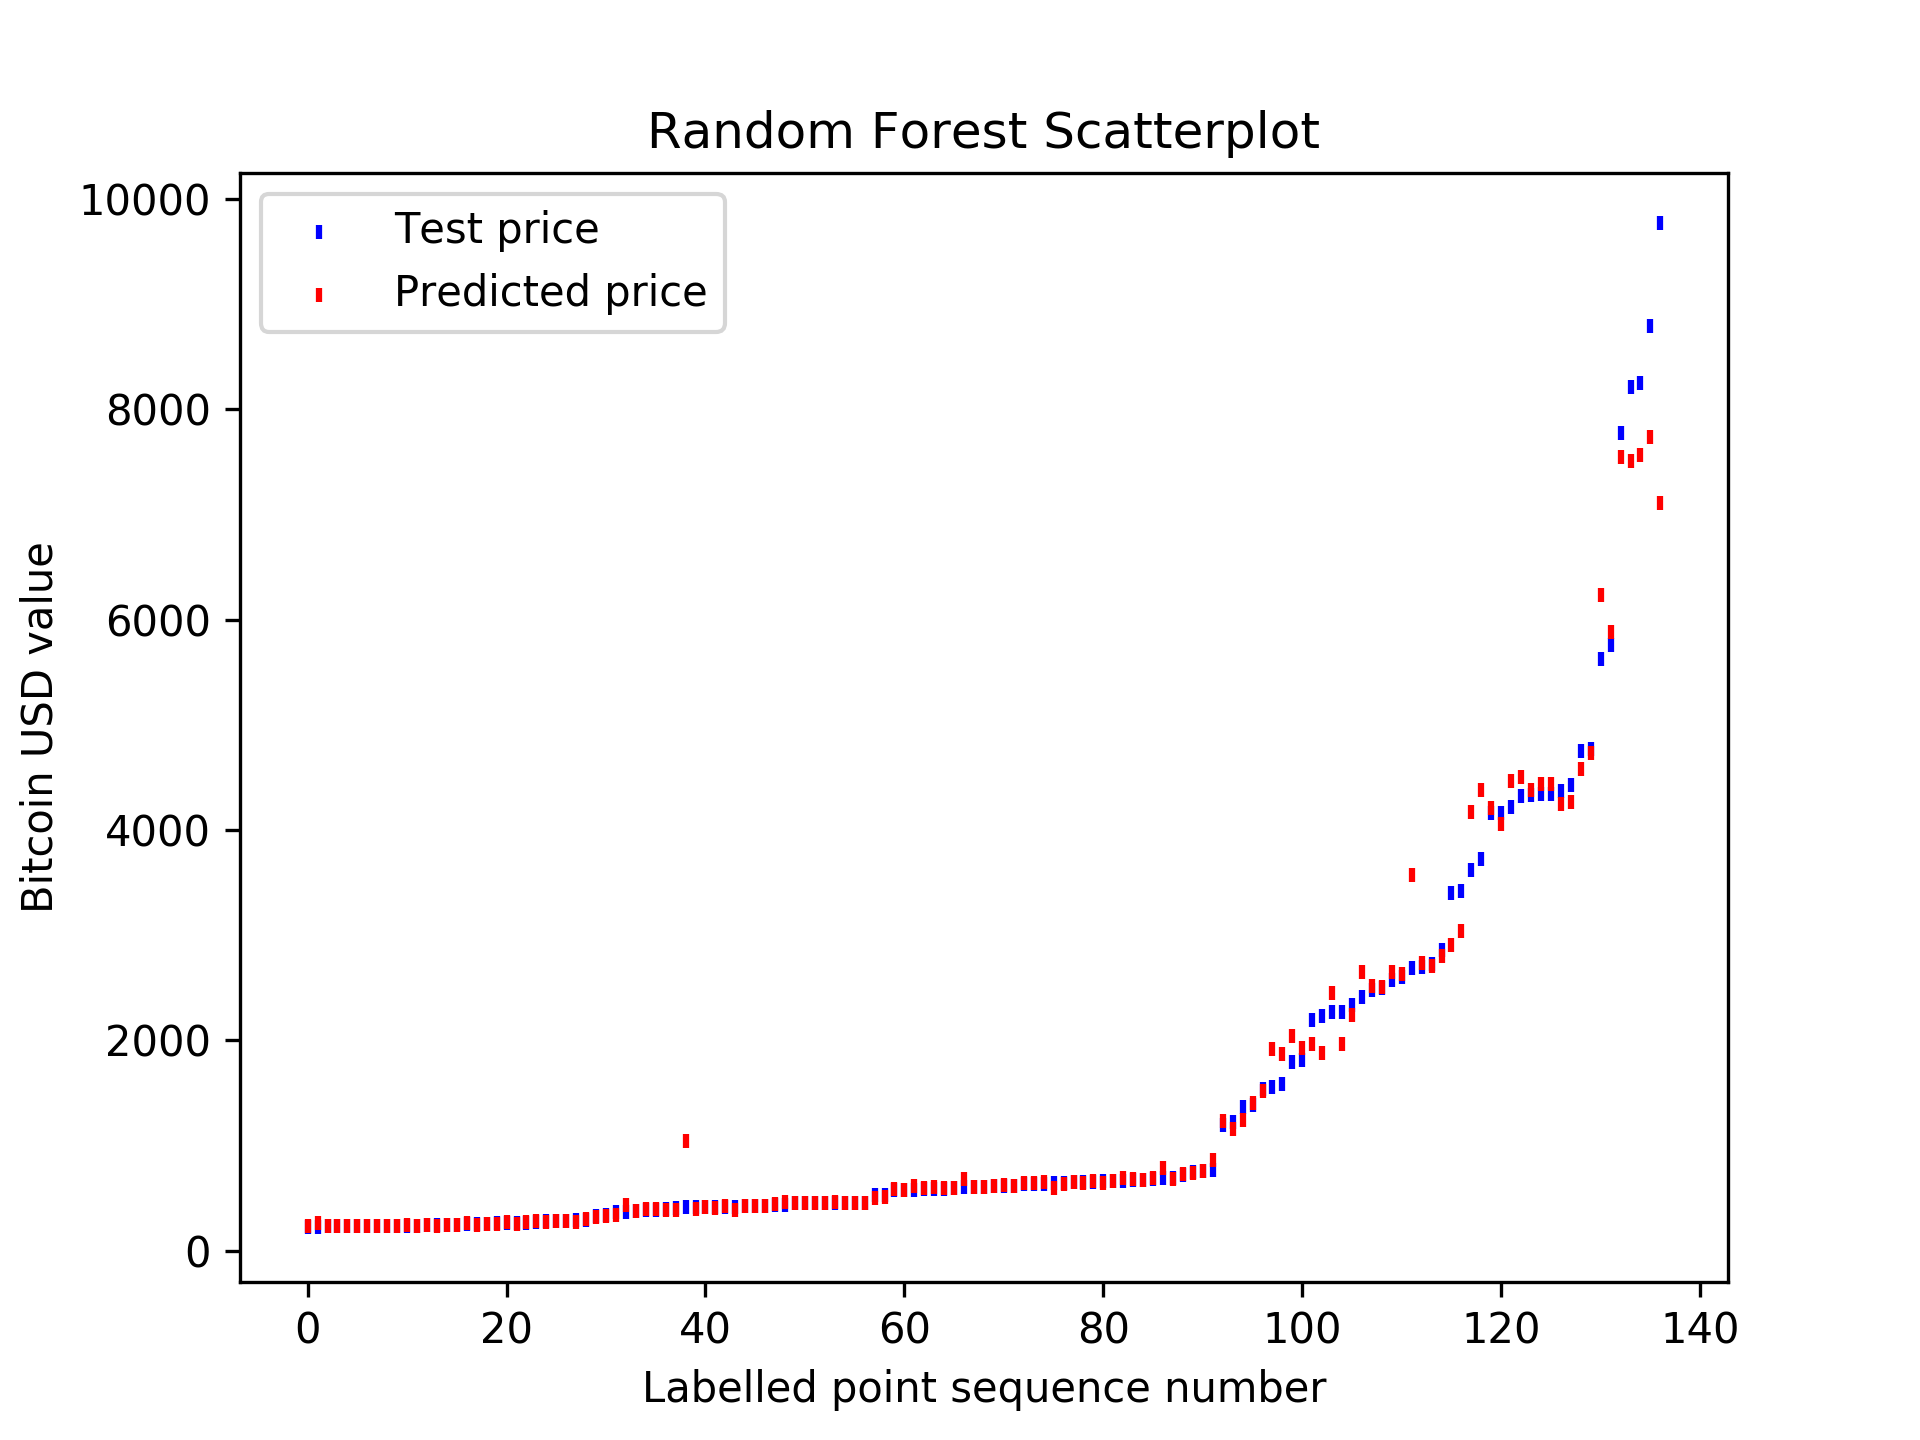
\includegraphics[width=\columnwidth]{images/RandomForestscatterplot.png}
  \caption{Randomforest Scatterplot}
  \label{scpl:ran}
\end{figure}

\begin{figure}[!ht]
  \centering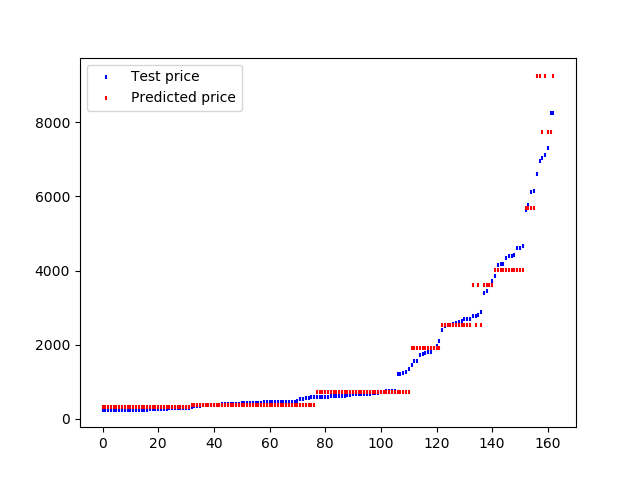
\includegraphics[width=\columnwidth]{images/GBTscatterplot.png}
  \caption{GBT Scatterplot}
  \label{scpl:gbt}
\end{figure}


From the observation of scatter plots of regression model Random forest \ref{scpl:ran} and GBT \ref{scpl:ran}, it is evident that GBT's single tree iterative model has predicted the values with overfitting. Some predicted values are consistent with some particular time scope and changes happening in steps. The prediction distribution looks like a single line and not widespread. Whereas, in the Random forest, the predicted values are widespread and closely aligned. Also, the other correlation graphs explain that Bitcoin transaction count doesn't impact the Bitcoin's values. even the exchange data doesn't impact much though the correlation looks close, there is a possibility that owners are not using the Bitcoin for any day to day transactions instead they are using as an asset like Gold, and by retaining it, the demand for the Bitcoin coin further increases. Also, the new-coins can only be generated through mining and the growth is controlled, coins in circulation keep reducing, increasing its cost.
This analysis clearly proves that Bitcoin bought are saved in the wallets are not used in the regular transaction much. Most of the Bitcoin's are retained to earn the profit over its demand and its growth.


\section{Challenges faced}
Most of the challenges are with the data and casting to the required data types as the correlation and regression functions need data either in Float or double data types. And handling all these constraints along with Big data specifics in mind adds up to the challenge, thanks to Apache Spark which handles the data lineage and persistence through RDDs.

\section{Project structure}
Three folders are created, the first one is for scripts which retain the actual code to be executed and two Korn shell scripts to install dependencies and to download the files. The second one is the data folder which retains the data required for the model and correlation algorithm. And the extracted folder is to persist the plot figures extracted out of the python script. And git is used to controlling the versioning of the project. 

\section{Improvement Opportunities}
There are a lot of improvement opportunities to be implemented in the project. One of them includes fetching the data in near real-time directly from the Mining-pool instead of a third party data service, the second one would be increasing the granularity of data which would increase the performance and  Spark make more sense with that level of granularity and volume. The other improvement opportunities include gathering more features like illegal market transaction data, mining exchange data, wallet exchange data, world's inconsistency data which will increase correlation factors and result in the accurate prediction of models. Other visualization opportunity includes real-time presentation capabilities with Big data at the back end. Matplot API has minimal options for real-time reporting which can be upgraded.

\section{Conclusion}

With all prowess of Big data and its technologies, Blockchain technologies are not only evolving, it also equips humans with the opportunity to make the world more transparent, ethical and a viable place to live. Even these technologies help us to conserve the earth by reducing resource consumption like paper, audit trials and power. As the technology has evolved so far, it is expected to understand its growth story in terms of its microscopic level to push it to the next level of improvement. Such microscopic level of qualities was missed in legacy methods and Big data comes to the rescue in identifying those qualities and nurturing them.


\begin{acks}
  The authors would like to thank Dr. Gregor von Laszewski for his support and suggestions to write this paper.
\end{acks}

\bibliographystyle{ACM-Reference-Format}
\bibliography{report} 



\end{document}
